\section{Introduction}

At some point in their academic journey, every student faces the challenge of selecting the elective courses required for graduation. Choosing the right "free choice" exam is difficult for several key reasons:

\begin{itemize}
	
	\item \textbf{Informative gap}: a major hurdle is the lack of up-to-date and relevant information regarding course material, examination formats, and the actual workload involved. Without these details, making an informed decision is nearly impossible.
	
	\item \textbf{Community experience}: the opinions of former students are essential for determining if a course aligns with one's academic goals and timeline. Unfortunately, it is often difficult to locate peers on campus or in online chats who are available to provide honest, detailed answers about specific subjects.
	
	\item \textbf{Professor competence}: the quality of a course is largely determined by a professor's teaching ability and their availability to students. It is nearly impossible to gauge a professor’s effectiveness without attending their lectures; however, this information is needed at the start of the semester, not at the end, when study plans are already locked and time has run out.
	
\end{itemize}

The solutions to all these problems is \textbf{EduMeter}, a platform made for students by students. 

\subsection{Statement}

\textbf{EduMeter} is a web platform dedicated to the students enrolled in a bachelor or master degree at the University of Florence for the view and publication of reviews on taken courses. \\

The system provides 3 types of entities: \textbf{guest user} (unauthenticated users), \textbf{student user} (authenticated user) and \textbf{admin}. Each entity is able to perform different and exclusive actions on the system data record. Here it is the descriptions of each entity possibility:

\begin{itemize}

    \item \textbf{Guest User}: this type of user is able to visualize the entire collection of reviews without authentication. It is possible to apply filters on the fields of the review body in order to navigate easily. 
	
	\item \textbf{Student User}: a student can authenticate with his personal institutional email, having his identity anonymized. Then he can navigate the review corpus and, additionally, he can post new reviews.
	
    \item \textbf{Admin}: this super user has the duty to perform the verification of the informations inserted by the student users in their reviews and accordingly operate the CRUD operations on the data records.  

\end{itemize} 

\vspace{.7em}
		
\begin{figure}[H]
	
	\centering
	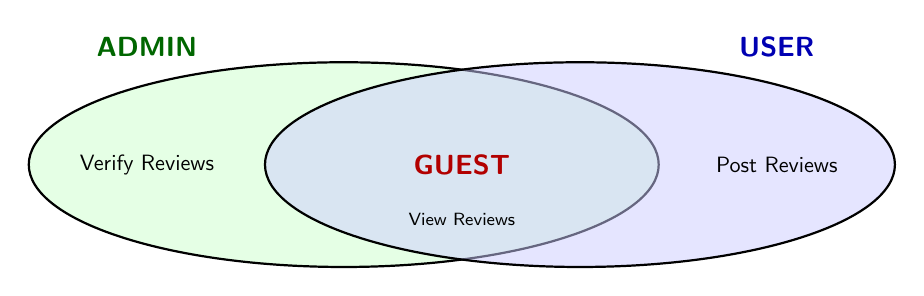
\begin{tikzpicture}[thick, font=\sffamily]
		
		% 1. ADMIN Ellipse (Left - Green)
		\draw[fill=green!20, fill opacity=0.5] (0,0) ellipse (4cm and 1.3cm);
		\node[text=green!40!black] at (-2.5, 1.5) {\textbf{ADMIN}};
		
		% 2. USER Ellipse (Right - Blue)
		\draw[fill=blue!20, fill opacity=0.5] (3,0) ellipse (4cm and 1.3cm);
		\node[text=blue!70!black] at (5.5, 1.5) {\textbf{USER}};
		
		% 3. GUEST Label (Placed in the intersection)
		% The intersection center is roughly at (1.5, 0)
		\node[text=red!70!black] at (1.5, 0) {\textbf{GUEST}};
		
		% --- Example Permissions ---
		\node[scale=0.8] at (-2.5, 0) {Verify Reviews}; % Admin Only side
		\node[scale=0.8] at (5.5, 0) {Post Reviews};   % User Only side
		\node[scale=0.8] at (1.5, -0.7) {\footnotesize View Reviews}; % Guest (Intersection)
		
	\end{tikzpicture}
	\caption{Permission Overlap}
	
\end{figure}

Each review has a fixed structure composed by numerical and string fields, the student has to fill them in order to post a the review. The fields are: \textbf{degree enrolled} (string), \textbf{reviewed course} (string), \textbf{teacher} (string), \textbf{year of completion} (number), \textbf{grading} (number), \textbf{comment} (string).
